\section{Energy Benchmarking}
\label{sec:energy}

Energy consumption has quickly become a critical dimension of machine learning benchmarking. Training and inference with modern AI systems can require enormous computational resources. Training a single large-scale language model can consume megawatt-hours of electricity, often rivaling the annual energy consumption of households.  
To illustrate the issue, we have provided in Table \ref{tab:energy-chatgpt} the energy required to train various ChatGPT models (some of which are projected, as no concrete data has been released). Additionally, we have included the energy cost for one million inference calls.

Here, training energy refers to total estimated power consumption during model training; inference energy represents the approximate power required for one million user queries. Values are derived from public estimates and projections—OpenAI has not released official figures \cite{sciencefeedback2024energy,kaplan2020scaling}. GPT-3 took roughly 1287 MWh to train~\cite{patterson2021carbon}, which is roughly equivalent to the annual power consumption of 130 homes in the US~\cite{WECEnergy}. 

For DOE leadership class machines, such as those hosted at Oakridge National Laboratory (see Table \ref{tab:ornl-energy}), we find documented and significant progress toward exascale but at the cost of increased energy consumption that more than doubled in the last generational upgrade. However, the Peak Performance per energy unit has significantly increased, and compared to the initial values from Jaguar, Frontier has improved by a factor of 209.


\begin{table}[tb]
\centering
\caption{Estimated Energy Consumption of GPT Models for Training and Inference 
(based on \cite{brown2020language, patterson2021carbon, medium2023gpt4carbon, 
extremenetworks2023energy, epochai2024compute, hackernoon2024dirtysecret}).}
\label{tab:energy-chatgpt}
\resizebox{\columnwidth}{!}{
\begin{tabular}{|l|c|c|}
\hline
\textbf{Model} & \textbf{\makecell{Training Energy\\(MWh)}} & \textbf{\makecell{Inference Energy\\(per 1M queries, MWh)}} \\
\hline
\hline
GPT-3 & $\sim$1,287 \cite{baeldung2023energy,patterson2021carbon} & $\sim$50--100 \\
\hline
GPT-4 & 51,773--62,319 \cite{medium2023gpt4carbon,extremenetworks2023energy} & $\sim$600--1,000 \\ \hline 
GPT-5 & $>$60,000 (estimated) \cite{epochai2024compute,hackernoon2024dirtysecret} & $\sim$800--1,200 \\ \hline
GPT-6 & 80,000--100,000 (projected) \cite{epochai2024compute} & $\sim$1,000--1,500 \\ \hline
\end{tabular}
}
\end{table}

\begin{figure}[tb]
    \centering
    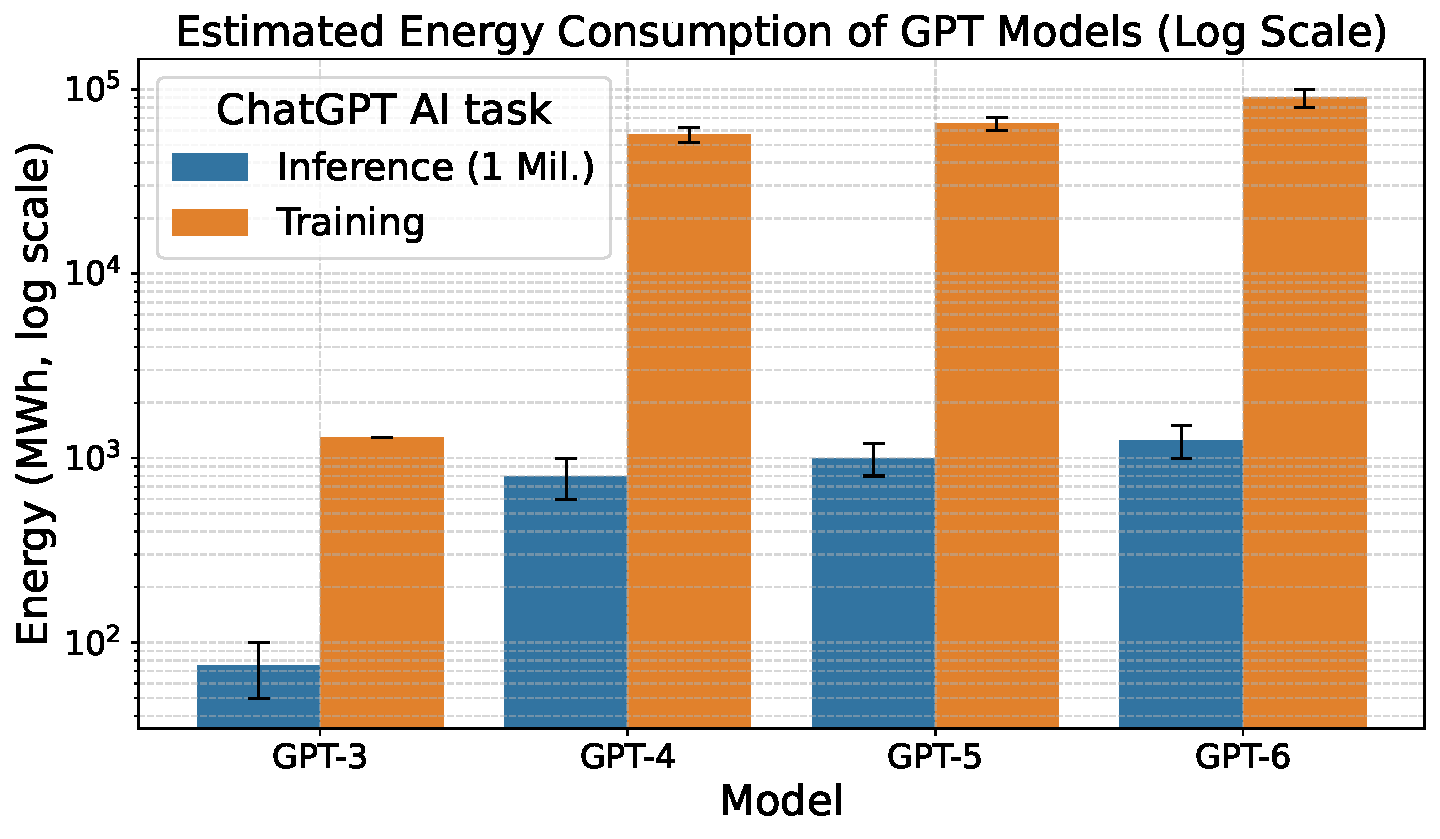
\includegraphics[width=1.0\linewidth]{images/gpt_energy_comparison.pdf}
    \caption{Energy consumption for training ChatGPT and inferencing 1 Million queries.}
    \label{fig:placeholder}
\end{figure}


\begin{table}[tb]

    \caption{Evolution of the leadership class supercomputer at Oak Ridge National Laboratory}
    \label{tab:ornl-energy}
    
    \resizebox{\columnwidth}{!}{
        \begin{tabular}{|l|c|l|r|r|r|}
            \hline
            \textbf{Machine} & \textbf{Year} & \textbf{Architecture} & \textbf{\makecell{Peak \\ Performance\\(PF)$^*$}} & \textbf{\makecell{Power\\ (MW)}} & \textbf{\makecell{Performance/\\Power\\(PF/MW)}} \\
            \hline
            \hline
            Jaguar   & 2009 & Multi-core CPU & 2.3   & 7  & 0.33 \\
            \hline
            Titan    & 2012 & Hybrid CPU/GPU & 27    & 9  & 3.00 \\
            \hline
            Summit   & 2017 & Hybrid CPU/GPU & 200   & 13 & 15.38 \\
            \hline
            Frontier & 2021 & Hybrid CPU/GPU & 2000  & 29 & 68.97 \\
            \hline
        \end{tabular}
    }

    \smallskip
    {\tiny~~ $^*$PF=\emph{peta–floating-point operations per second}; $1\;\text{PF}=10^{15}\text{FLOPS}.$

    ~~~ Data derived from \cite{papatheodore2022summitfrontier}.
    }
\end{table}

Having a more detailed understanding of the impact on energy is today also been measured in carbon emissions. 

\begin{comment}
The following examples highlight this issue and have direct impact into budget and sustainability decisions.

\noindent
\textbf{Case 1 – Oak Ridge’s \emph{Frontier}.} %
The Frontier exascale system draws
\(24.6\;\text{MW}\) at LINPACK load and is housed in a data hall whose measured PUE is \(1.03\)\,\cite{DOE_Frontier_Power2023}. At the July 2025 U.S.\ industrial tariff of
\$0.081 kWh\(^{-1}\)\,\cite{EIA_Electricity_Price_2025} the annual electricity bill is: $24.6\;\text{MW}\times 8\,760\;\text{h\,yr}^{-1}\times\$0.081
  \;\approx\;\$17.5\,\text{M}/\text{yr}.$  The Tennessee Valley Authority reported a residual grid intensity of
\(360\;\text{g\,CO}_{2}\text{e\,kWh}^{-1}\) for 2024\footnote{TVA
Sustainability Report (2025), \url{https://tva.com/environment/environmental-stewardship/sustainability}.} so Frontier emits
\(\sim\!78\;\text{kt\,CO}_{2}\text{e\,yr}^{-1}\), equivalent to the
territorial footprint of \(\sim\!12\,000\) EU residents
(Eurostat 2024, 6.5 t cap\(^{-1}\))\,\cite{Eurostat_GHG_2024}.

%\vspace{4pt}
\noindent
\textbf{Case 2 – Google hyperscale fleet.} %
Google’s 2023 environmental report lists a \emph{fleet-wide} PUE of
\(\mathbf{1.10}\) (industry mean 1.58)\,\cite{Google_PUE_2023} yet company-wide GHG emissions still rose to
\(14.3\;\text{Mt\,CO}_{2}\text{e}\) in 2023, up 49 \% since
2019\,\cite{Google_Sustainability_2024}.   % <5>
Internal modeling shows that deferring non-urgent ML jobs to periods of
low grid-carbon intensity cuts emissions by 10–20 \%; Google plans to
combine that policy with a 115 MW geothermal PPA coming online in Nevada
in 2026\,\cite{Google_Geothermal_2023}.   % <6>

\end{comment}

If we only focus on traditional benchmarks using metrics such as FLOPS or latency, we provide performance insights but overlook {\em energy-to-solution}, which measures the total energy required to complete a task. Without perspective, researchers and practitioners focus on optimizing for speed at the expense of sustainability and cost efficiency. 

Thus, we believe it is important to make energy benchmarks an important aspect of AI benchmarks. Energy benchmarking ought to address the following:

\begin{itemize}
     \item Quantify the environmental footprint of AI workloads (carbon emissions, renewable vs. non-renewable energy use).
     \item Highlight economic tradeoffs in large-scale computing (cloud costs, datacenter efficiency). 
     \item Guide hardware and algorithmic choices towards a more effective architecture.
     \item Support policy and funding decisions by providing transparent data on sustainability. 
 \end{itemize}

Energy-aware benchmarks help ensure that AI development aligns with broader goals of responsible computing, making results reproducible, performant, and economically and environmentally sustainable. 

Thus, we see several opportunities. First, we need to make energy benchmarks more prominent and provide materials and tutorials as part of AI benchmark carpentry to educate the community. Second, we must make sure that not only the most expensive hardware, such as leadership class and hyper-scale data centers, are used, but also medium-scale and even small-scale so that democratizing energy benchmarks in the community is easy to do and execute. This way, measurements of even smaller AI-based scientific applications can integrate energy consumption in their benchmarks, and meaningful comparisons to even traditional algorithms that do not use AI can be drawn. Third we must make sure that energy metrics and logs can be accessed and integrated in a uniform way into the AI benchmarks.

\subsection{AI energy benchmark carpentry}

To support AI energy benchmark carpentry efforts, we need to address the following issues:

\begin{itemize}
\item Conduct a relevant survey of existing efforts
\item Identify Metrics useful for AI benchmarks 
\item Identify how to leverage existing and create new leaderboards focusing on energy metrics
\item Identify simple to use blueprints as part of the carpentry efforts that can be replicated and reused, as well as serve as a basis for newly developed benchmarks.
\item conduct community outreach to offer carpentry tutorials that focus on AI benchmarks instead of just AI software and services.
\item identify how to obtain and integrate meaningful and practical metrics (example: data centers may not provide uniform access to energy data). Thus, energy data collection and access must be part of the carpentry efforts.
\end{itemize}

Strategies to integrate energy into AI benchmarks for  carpentry efforts included improving access to metrics for democratizing them, including creating logs during runtime, focusing on:

\begin{itemize}
    \item Logging ambient temperature and humidity.
    \item Logging sample power at regular intervals or averages over the run.
    \item Store the logging data in an easy-to-parse format (CSV, JSON, YAML) 
    \item Upload results as artifacts in support of the FAIR principle and make available for comparison.
\end{itemize}

Next, we discuss some of the aspects that need to be addressed in more detail.


\subsection{Energy Metrics.}

There are various energy metrics that one can consider. The community may not be aware of them, and a need exists to provide such information. It is also important to identify metrics that can be used in leaderboards for comparison, but they must be obtained in a manner that allows fair and informed comparisons. Hence, documenting how the experiment needs to be conducted is imperative instead of just referring to the metric. In principle, blueprints should be used and adapted to make the comparison across hardware and software more easily possible. Energy metrics are used on different layers of the infrastructure used in AI benchmarks, which is similar to classical HPC infrastructure. We provide an example of using different metrics on the various layers in Figure \ref{fig:energy-metric-layer}. Such diagrams should be integrated into the blueprints provided to the users to simplify understanding the scope of the benchmarks in regard to energy.

\FINPUT{graph-energy-layered.tex}


As part of the energy augmentation, a clear purpose for the benchmark metric should be stated. 
Such examples should be collected as part of the metadata of the experiment so they can be leveraged and be a motivator for other benchmarks.  In our example from Figure \ref {fig:energy-metric-layer}, the purpose for each metric is as follows:

\begin{itemize}

\begin{enumerate}[label=\arabic*., leftmargin=0pt, labelsep=1em, align=left]

\item Device/Microarchitectural Layer
\begin{itemize}
        \item \textbf{Energy per flop} or \textbf{Energy per inference}: Measures the energy consumed to perform a single computational operation (a floating-point operation or an inference).
        \item \textbf{Temperature sensors}: \emph{Related Logging (Non-KPI):} \textbf{Inlet and Outlet Temperature Sensors}: Logged because \textbf{thermal headroom} directly bounds the safe \textbf{Dynamic Voltage and Frequency Scaling (DVFS)} ranges.
\end{itemize}
\item Job/System Layer
\begin{itemize}

        \item \textbf{Kilowatt-hour (kWh)}: The total energy consumed by a specific job or set of jobs over its duration.
        \item \textbf{Energy--Delay Product (EDP)}: A combined metric of energy and time (energy $\times$ delay) used to assess the overall efficiency of a computation. Lower EDP generally indicates better performance and efficiency.
\end{itemize}

\item Facilities/Data Center Layer
\begin{itemize}

        \item \textbf{Power Usage Effectiveness (PUE)}: A ratio that measures how efficiently a data center uses energy. An ideal PUE is 1.0 (meaning all energy goes to the IT equipment).
        \textbf{Data Center Infrastructure Efficiency (DCiE)}: The reciprocal of PUE, expressed as a percentage. It shows what percentage of the total data center energy is actually used by the IT equipment.
\end{itemize}

\end{enumerate}
\end{itemize}

This tiered structure, along with a detailed purpose statement for each metric, allows for meaningful comparisons and decision-making at every level of the computing infrastructure.

To identify commonly used metrics, we conducted an initial survey of tools and benchmarks related to energy that we display in Table \ref{tab:hpc_energy_catalog}.
We list the core metrics, as well as their typical benchmark use.

Common requirements for such metrics include obtaining the measurements in a low-cost fashion, sharing the results with metadata augmentations, and integrating them into potential leaderboards. 
We believe we have to go beyond established Leaderboards such as \textbf{Green500} and the \textbf{MLPerf Power}, which already influence processor road-maps and procurement calls~\cite{Scogland11Green500,Tschand24MLPerfPower}, as to raise awareness of the energy impact on real-world scientific applications.

\subsection{Leveraging previous work}

As we can see from the table, a large number of tools and benchmarks exist, and we can leverage from them to work towards a FAIR-based approach on energy benchmarks. This is all the more important when developing concise carpentry and democratization efforts. The distinction in the layered architecture for energy benchmarks also helps, as it is in many cases not possible or desirable to address all of the layers at once. It is obvious that energy benchmarking in itself is a complex research topic and that carpentry efforts must be established to bring this knowledge forward and enhance AI benchmarks to AI energy benchmarks.

\begin{comment}

\TODO{this may be possible to be integrated in the table as a column, where we note on which level the benchmark is, that seems real useful}

\emph{One scalar per machine}—ideal for non-experts and procurement:
\textsc{SPECpower\_ssj2008}, \textsc{SERT2}, \textsc{TPC-Energy}, \textsc{JouleSort}, \textsc{Green500}, \textsc{HPCG-Power}, \textsc{HPL-MxP}, \textsc{MLPerf Power}, and \textsc{MLPerf Tiny}.
Their scores appear in vendor brochures, ENERGY-STAR dossiers, and EU Lot 9 conformity reports~\cite{EU_Lot9_Guidance}. %% EU2019_424,

\paragraph{Instrumentation frameworks.}
\TODO{What is an instrumentation framework}

Calibrated telemetry collectors—\textsc{SPEC PTDaemon}+RAPL/NVML, \textsc{Scaphandre}, \textsc{Kepler}, IBM \textsc{PowerAPI}, NVIDIA
\textsc{DCGM Energy}, Intel \textsc{VTune Power}, Cray \textsc{PAT Energy}—provide the 1 Hz power traces that optimization research needs.

\paragraph{Mini-apps and carbon wrappers.}
\TODO{What are Mini-apps and carbon wrappers.}
Power-augmented kernels (\textsc{LULESH-Power}, \textsc{CosmoFlow-Power}, \textsc{GROMACS-EE}, \dots) and wrappers (\textsc{CodeCarbon}, \textsc{CarbonTracker}) translate joules into kg CO\(_2\)e or cost, completing the silicon-to-sustainability loop.

\end{comment}


\begin{table*}[hptb]
  \centering
  \caption{
  Energy- or carbon-efficiency benchmarks (B) and tools (T) used in scientific-HPC research.  Metrics use ``/'' for ``per''; ``;'' separates multiple items; ``+'' appears only where a spec explicitly combines two values into one score
  %Benchmarks, tools, and initiatives that publish energy‑ or carbon‑efficiency metrics for Scientific‑HPC workloads.
  }
  \label{tab:hpc_energy_catalog}
  %\renewcommand{\arraystretch}{1.1}
  %\setlength{\tabcolsep}{4pt}
  \rowcolors{2}{white}{lightgray}
  \begin{tabularx}{1.0\textwidth}{|llllX|}
    \toprule
    & \headerfont\textbf{(B)enchmark or (T)ool}
    & 
    & \headerfont\textbf{Core metric(s) } %\& data captured} 
    & \headerfont\textbf{Typical Benchmarking Use}\\ 
    \midrule
B & SPECpower\_ssj2008           & \cite{specpower}            & W/transaction; ops/W                & Enterprise-server rankings; ENERGY STAR compliance \\
B & SPEC\,SERT$^{2}$             & \cite{sert2}                & Server-Efficiency-Rating = kWh + perf    & EU Lot 9 certification; vendor datasheets \\
B & TPC-Energy                   & \cite{tpcenergy}            & Wh/DB phase                            & OLTP/warehouse energy cost studies \\
B & JouleSort                    & \cite{joulesort}            & records/J                              & Storage-I/O contests; I/O-stack tuning \\
B & Green500                     & \cite{green500}             & GFLOPS/W (HPL or HPL-AI)               & Global supercomputer energy ranking \\
B & HPCG-Power                   & \cite{hpcgpower}            & GFLOPS/W (HPCG)                        & Memory-bound tuning; procurement add-on to TOP500 \\
B & HPL-MxP (HPL-AI)             & \cite{hplmxphplai}          & mixed-precision GFLOPS/W               & GPU/TPU evaluation for AI-optimised LINPACK \\
B & MLPerf Power                 & \cite{mlperfpower}          & J; avg W; J/sample; J/epoch       & Official energy track for MLPerf submissions \\
B & MLPerf Tiny                  & \cite{mlperftiny}           & $\mu$J/inference (MCU)             & Edge-AI board comparison; ultra-low-power design \\
B & CoreMark-PRO Power           & \cite{coremarkpro}          & iterations/s/W (SoC)                 & Pre-silicon DVFS sweeps; embedded RFPs \\ 
B & UL Procyon AI Power          & \cite{procyon}              & images/W; fps/W                     & Smartphone \& laptop AI-inference benchmarks \\
B & CANDLE Power Study           & \cite{candlepowerstud}      & J/epoch; GFLOPS/W                   & DOE accelerator procurement guidance \\
B & LULESH/miniFE Energy       & \cite{luleshminifeene}      & J/iteration                            & DVFS + autotuning baselines \\
B & ExaSMR Power Benchmark       & \cite{exasmrpowerbenc}      & J/neutron; energy-vs-accuracy curve   & Energy budget strategy in nuclear simulations \\
B & EE-HPC-WG Energy Benchmark   & \cite{eehpcwgenergybe}      & draft node/job spec; JSON trace       & Toward common HPC energy standard \\
B & HPC-AI500 Energy Track       & \cite{hpcai500energyt}      & planned: GFLOPS/W; tokens/J         & Mixed AI/HPC cluster evaluations \\
B & PARSEC-3.1 Energy Extension  & \cite{parsec31energye}      & W; J via PAPI-RAPL; J/op; EDP       & Pre-silicon DVFS research \\
B & CosmoFlow-Power              & \cite{cosmoflow2019}        & J/epoch; GFLOPS/W                   & CNN scaling on 15 k+ GPUs \\
B & HACC Energy Add-on           & \cite{hacc2020power}        & J/particle update                      & N-body cosmology power studies \\
B & DeepCAM-Energy               & \cite{deepcam2020power}     & J/epoch (UNet)                         & Climate-analytics accelerator studies \\
B & OpenIFS-Energy               & \cite{openifsenergy2023}    & kWh/model-day; W timeline             & Weather-model node comparison \\
B & GROMACS-EE                   & \cite{gromacsee2024}        & J/ns; W/GPU                         & MD clock-vs-accuracy trade-offs \\
B & NAMD-Power                   & \cite{namdpower2019}        & Energy-Delay-Product (ApoA1)             & Summit node DVFS optimisation \\
B & QE Energy Suite              & \cite{qeenergy2022}         & J/SCF step; GFLOPS/W                & DFT GPU-offload studies \\
B & VASP-Power Harness           & \cite{vasppower2023}        & W; kWh/MD step                        & Materials-science accelerator compare \\
B & OpenFOAM-Energy              & \cite{openfoamenergy2021}   & J/1k iterations                       & CFD partitioning \& mesh tuning \\
B & InSAR-AI Power Kit           & \cite{insarpower2024}       & J/satellite scene                      & Edge-to-cloud EO inference cost \\
B & H3D-Energy                   & \cite{h3denergy2023}        & J/hydrology timestep                & Hydrology model DVFS exploration \\ \hline\hline  
T & PTDaemon/SERT Energy       & \cite{specptdaemonser}      & calibrated W; kWh (node)                & Lab reproducibility; Lot 9 labels \\
T & Scaphandre                   & \cite{scaphandre}           & W; kWh (process/node, Prometheus)     & Slurm dashboards; power-cap feedback \\
T & Kepler                       & \cite{kepler}               & W/pod; J/pod (eBPF)                 & Energy observability in K8s clusters \\
T & CodeCarbon                   & \cite{codecarbon}           & kWh; kg CO\(_2\)e (process)             & Rapid CO\(_2\) estimation in pipelines \\
T & CarbonTracker                & \cite{carbontracker}        & measured + predicted kWh; CO\(_2\)e     & Scheduling DL jobs in low-carbon hours \\
T & PowerPACK/Mont-Blanc       & \cite{powerpackmontbl}      & W; J for MPI/OpenMP mini-apps         & Network-topology \& DVFS studies \\
T & Cray PAT Energy Counters     & \cite{craypatenergyco}      & J/function; avg W                     & Kernel hotspot hunting on Shasta \\
T & IBM PowerAPI (pmlib)         & \cite{ibmpowerapipmli}      & kWh (job/process)                      & Energy-aware scheduling on Summit \\
T & NVIDIA DCGM Energy           & \cite{nvidiadcgmenerg}      & W; J (GPU) \@ 1Hz; telemetry           & GPU power-cap discovery; Green500 \\
T & Intel VTune Power            & \cite{intelvtunepower}      & package W; J/function                 & Roofline-vs-energy tuning on Xeon \\ 

\bottomrule   
  \end{tabularx}
\end{table*}


 
 
 %  B & SPECpower\_ssj2008 & \cite{specpower}            & Watts per transaction; ops/W & Enterprise‑server energy rankings and ENERGY STAR compliance \\  
 % B  & SPEC SERT$^{2}$  & \cite{sert2}                   & Server Efficiency Rating (kWh+perf)& Lot 9 regulatory testing; vendor datasheets \\  
 % B  & TPC‑Energy  & \cite{tpcenergy}                    & Watt‑hours per database phase & Energy‑cost analysis for OLTP/warehousing appliances \\  
 % B  & JouleSort  & \cite{joulesort}                     & Records per Joule  B  & Storage‑I/O hardware contests; I/O stack optimisation \\  
 % B  & Green500  & \cite{green500}                       & GFLOPS/W (HPL/HPL‑AI) & Global supercomputer energy‑efficiency ranking \\  
 % B  & HPCG‑Power  & \cite{hpcgpower}                    & GFLOPS/W (HPCG) & Memory‑bound workload tuning; procurement add‑on to TOP500 \\  
 %  B & HPL‑MxP (HPL‑AI)  & \cite{hplmxphplai}            & Mixed‑precision GFLOPS/W & AI‑optimised LINPACK evaluation for next‑gen GPUs/TPUs \\  
 %   B & MLPerf Power  & \cite{mlperfpower}                & Joules, avg W; J/sample or J/epoch & Official energy track for MLPerf submissions (training + inference) \\  
 %   B & MLPerf Tiny  & \cite{mlperftiny}                  & $\mu$J/inference on MCU & Edge‑AI board comparisons; ultra‑low‑power design \\  
 %  B & CoreMark‑PRO Power  & \cite{coremarkpro}          & Iterations/s/W for SoCs & Pre‑silicon DVFS sweeps; embedded RFPs \\  
 %  B & UL Procyon AI Power  & \cite{procyon}             & Images/W; fps/W \& Smartphone & laptop AI inference benchmarks \\  
 %   B & CANDLE Power Study  & \cite{candlepowerstud}      & Joules/epoch; GFLOPS/W for ResNet‑50 & DOE accelerator procurement guidelines \\  
 %  B & LULESH/miniFE Energy  & \cite{luleshminifeene}    & Joules per iteration & Baseline for DVFS + autotuning papers \\  
 %  B & ExaSMR Power Benchmark  & \cite{exasmrpowerbenc}  & Energy vs neutron‑transport accuracy & Energy budget strategy in nuclear simulations \\  
 %  B & EE‑HPC‑WG Energy Benchmark  & \cite{eehpcwgenergybe}& Draft node/job spec (JSON, RAPL|NVML) & Toward a common HPC energy standard \\  
 %  B & HPC‑AI500 Energy Track  & \cite{hpcai500energyt}  & Planned GFLOPS/W + tokens/J & Mixed AI/HPC cluster evaluations \\  
 %  B & PARSEC‑3.1 Energy Extension  & \cite{parsec31energye} & Watts \& Joules via PAPI‑RAPL; J/op, EDP & Pre‑silicon DVFS research \\  
 %  B & CosmoFlow‑Power  & \cite{cosmoflow2019}           & Joules/epoch; GFLOPS/W & Cosmology CNN scaling on 15k+ GPUs \\  
 %  B & HACC Energy Add‑on  & \cite{hacc2020power}        & Joules per particle update & N‑body cosmology power studies \\  
 %  B & DeepCAM‑Energy  & \cite{deepcam2020power}         & Joules/epoch for UNet cloud segmentation & Climate analytics accelerator studies \\  
 %  B & OpenIFS‑Energy  & \cite{openifsenergy2023}        & kWh per model‑day; W timeline & Weather/climate node comparison \\  
 %  B & GROMACS‑EE  & \cite{gromacsee2024}                & Joules/ns; Watts/GPU & MD clock‑vs‑accuracy trade‑offs \\  
 %  B & NAMD‑Power  & \cite{namdpower2019}                & Energy‑Delay Product for ApoA1 & Summit node DVFS optimisation \\  
 %  B & QE Energy Suite  & \cite{qeenergy2022}            & Joules per SCF step; GFLOPS/W & DFT GPU‑offload studies \\  
 %  B & VASP‑Power Harness  & \cite{vasppower2023}        & Watts \& kWh per MD step & Materials science accelerator comparisons \\  
 %  B & OpenFOAM‑Energy  & \cite{openfoamenergy2021}      & Joules per 1k solver iterations & CFD partitioning \& mesh tuning \\  
 %  B & InSAR‑AI Power Kit  & \cite{insarpower2024}       & Joules per satellite scene & Edge‑to‑cloud EO inference cost models \\  
 %  B & H3D‑Energy  & \cite{h3denergy2023}                & Joules per hydrology timestep & Hydrology model DVFS exploration \\ 
 %  \hline
 %  \hline
 %  T & PEC PTDaemon/SERT Energy  & \cite{specptdaemonser} & Calibrated Watts/kWh per node & Lab‑to‑lab reproducibility; EU Lot 9 server labels \\  
 % T & Scaphandre  & \cite{scaphandre}                    & Process \& node Watts/kWh (Prometheus) & Job‑level carbon dashboards; power‑cap feedback in Slurm \\  
 % T & Kepler  & \cite{kepler}                            & Watts/Joules per K8s pod via eBPF & Energy observability in cloud‑native HPC \& AI clusters \\
 %   T & CodeCarbon  & \cite{codecarbon}                   & kWh
 %    \& kg CO\textsubscript{2}e per process & Rapid CO$_2$ estimation in research pipelines \\  
 %  T & CarbonTracker  & \cite{carbontracker}             & Predicted + measured energy/CO$_2$e & Scheduling long DL trainings to low‑carbon hours \\  
 %  T & PowerPACK/Mont‑Blanc  & \cite{powerpackmontbl}  & Joules \& Watts for MPI/OpenMP mini‑apps & Network topology \& DVFS studies without full apps \\  
 %   T & Cray PAT Energy Counters  & \cite{craypatenergyco}& Per‑function Joules and avg W & Hot‑spot hunting on XC/Shasta systems \\  
 %   T & IBM PowerAPI (pmlib)  & \cite{ibmpowerapipmli}    & Job \& process kWh streams & Energy‑aware scheduling on Summit/Sierra \\  
 %  T & NVIDIA DCGM Energy  & \cite{nvidiadcgmenerg}      & GPU Watts \& Joules \@ 1 Hz + telemetry & Optimal GPU power cap discovery; Green500 validation \\  
 %  T & Intel VTune Power Analysis  & \cite{intelvtunepower}& Package Watts; energy‑per‑function & Roofline‑vs‑energy tuning on Xeon/AMX CPUs \\  
 %  \bottomrule
  
%% CANDLE appears as a `C' because it is a published collection of measured results rather than a runnable code base




\begin{comment}
%----------------------------------------------------
\subsection{Energy Metrics}
\label{sec:energy-metrics}

\TODO{Old title is a bit too complex and mixes layers with concrete metric names, thus we can not use: Metric Layers, Temperature, and DCiE}

\TODO{Maybe we should say: As we can see form Table \ref{tab???} a plethora of energy related metrics exists. Software Carpentry and Democratizing efforts must educate users about them but also must possibly focus on the most useful or accepted once. Besides listing the actual energy used another important metric is the carbon emission. This is especially important is carbon emission as it has become world wide a measure for the impact on the environment. This motivates also many stakeholders to work towards zero carbon emission ... Think this over ...
Other metrics such as temperature, ... may be intermediate measurements if energy or carbon emission may not be immediately available.
}

\textit{Why it matters for carpentry.}  
\TODO{ i like the layer specific vs log but these are as you point out different things. SO one should look for what is measured and possibly establish the layer in a diagram and put the abstraction into it}
Layer-specific metrics tell authors \emph{what to log} and reviewers \emph{how to compare} submissions that run on very different hardware. Device-level energy per flop or inference pinpoints micro-architectural hot-spots; job-level kWh and Energy–Delay Product drive power-cap schedulers; facility-level PUE and DCiE satisfy CSR reporting. Although temperature is not itself a KPI, inlet and outlet sensors are logged because thermal headroom bounds safe DVFS ranges.

%------------------------------------------------------
\subsection{From On-Chip Counters to Carbon APIs} %% Instrumentation: 
\label{sec:energy:instr}

\textit{Why it matters for carpentry.} By funneling RAPL, NVML, and PM\_COUNTER readings through a uniform 1 Hz JSON trace, the kit ensures that the power data looks the same on a laptop or an exascale node. On-chip counters deliver sub-second energy samples; for leaderboard runs, these are cross-checked with an external power analyzer driven by \textsc{SPEC PTDaemon}. Cluster collectors (\textsc{Scaphandre},
IBM \textsc{PowerAPI}, NVIDIA \textsc{DCGM Energy}) stream calibrated data to Prometheus, and carbon wrappers (\textsc{CodeCarbon}, \textsc{CarbonTracker}) tag each joule with live grid-intensity kg CO\(_2\)e factors. Figure~\ref{fig:pipeline} shows the resulting
acquire $\rightarrow$ normalize $\rightarrow$ KPI flow.

\begin{figure}[!ht]
  \centering
  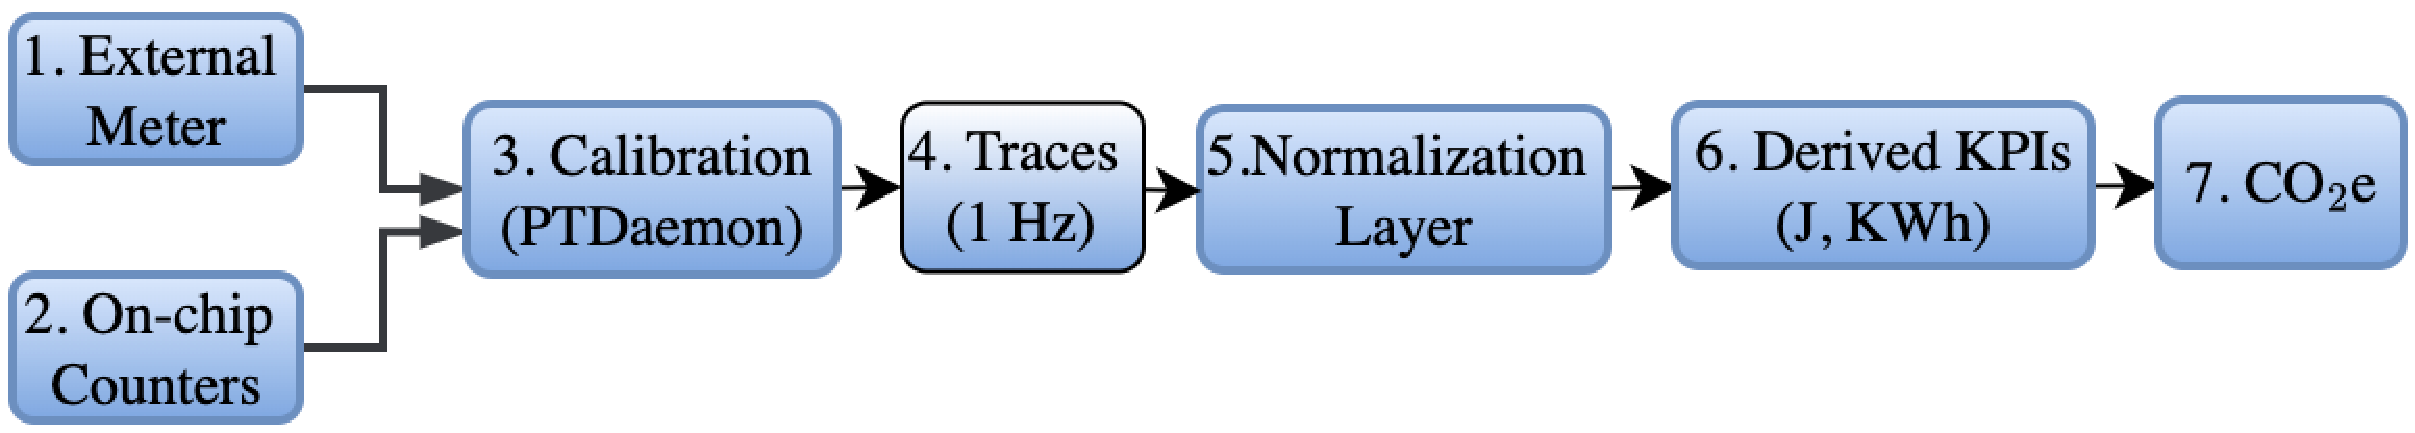
\includegraphics[scale=0.22]{images/kpi.pdf}
  \caption{Measurement workflow adopted by the energy-carpentry kit. Raw counter data are calibrated, normalized to J/kWh, converted to kg CO\(_2\)e via grid-intensity APIs, and aggregated into per-job KPIs. \TODO{this figure does not address the meter challang as the meters are on differnt levels. this seems to be here the application level not the center level. Also we have multiple meters ... the reason this seems incomplete is that on chip counter is on same level as external meter? Also we can plug in an external meter onto the CPU or GPU if we are real ambitious which I think has been done at SDSC. We do not need to mention this though ... as for this discussion to detailed. }}
  \label{fig:pipeline}
\end{figure}

%----------------------------------------------------------------------
\subsection{A Generalized Survey Framework}
\label{sec:energy:survey}

\textit{Why it matters for carpentry.}  
This three-stage template lets any new benchmark publish FAIR, trace-backed energy data with minimal extra code.

\begin{enumerate}[leftmargin=*]
  \item \textbf{Acquisition} — log 1 Hz power from counters \emph{and} a calibrated wall-plug meter.
  \item \textbf{Normalisation} — convert to J, kWh, kg CO\(_2\)e and derive GFLOPS/W, EDP, etc.
  \item \textbf{Reporting} — bundle traces + metadata in the \texttt{EE-HPC-WG} JSON schema and archive under a DOI.
\end{enumerate}

%----------------------------------------------------------------------
\subsection{Trade-offs and Scaling Limits}
\label{sec:energy:tradeoffs}

\textit{Why it matters for carpentry.}  
The kit lets any lab replicate these studies and contribute points to the communal dashboard. Capping an A100 at 300 W saves 11\%  energy for a 1\% speed loss~\cite{nvidiadcgmenerg}; HPL-MxP more than doubles GFLOPS/W over FP64~\cite{hplmxphplai}; CosmoFlow energy/epoch flattens beyond 8,000 GPUs
\cite{cosmoflow2019}. Figure~\ref{fig:tdp_scatter} contextualizes these results against historical CPU/GPU TDP trends.

\begin{figure}[ht]
  \centering
  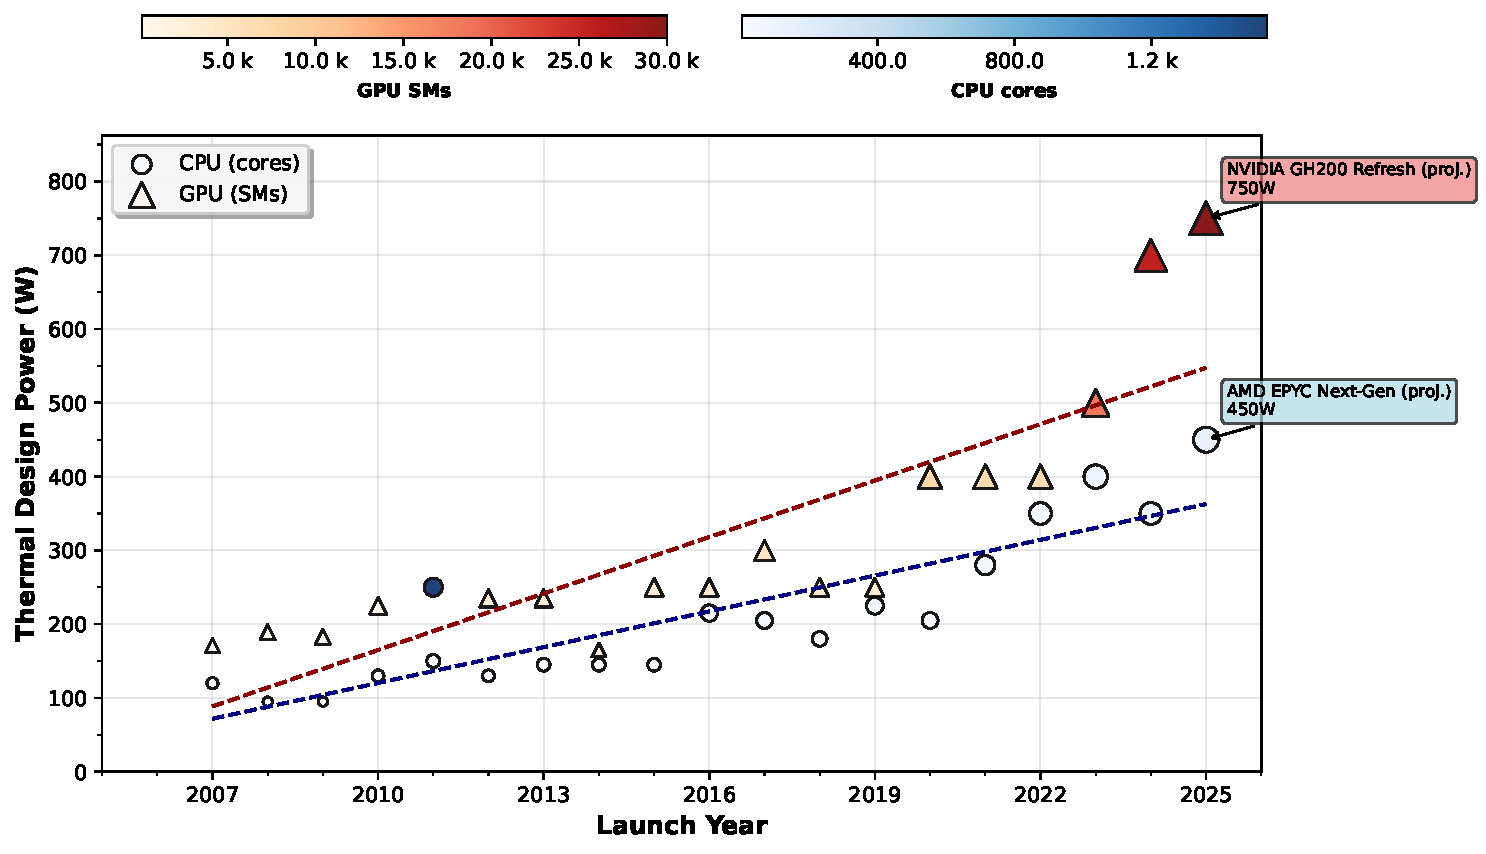
\includegraphics[width=\columnwidth]{images/tdp_vs_cpu-gpu.pdf}
  %\caption{Thermal-design power (TDP) and core/SM counts of flagship CPUs and GPUs, 2007–2025. Marker size~\(\propto\)TDP; color encodes parallel units. Linear fits show power budgets rising faster than on-chip parallelism.}
  \caption{\TODO{move this figure after the table from ORNL. and say this is what happens in the community. There is a citation missing where the data comes from... or is it self made? is the thermal design power important as we also consider flops. so should it be power/flops? to normalize, if so would that not be smaller in principal.} Evolution of flagship CPU and GPU power envelopes (2007–2025). Marker size scales with thermal design power (TDP); color encodes the advertised number of cores/SMs. The diverging linear trends reveal that peak power is growing faster than on-chip parallelism—a widening gap that any reproducible energy benchmark must capture and normalize if results are to remain portable across hardware generations.}
  \label{fig:tdp_scatter}
\end{figure}



%------------------------------------------------------
\subsection{Datacenter Benchmarks in Practice}
\label{sec:energy:dcbench}

\textit{Why it matters for carpentry.}  
Highlighting which suites dominate procurement reveals coverage gaps the community can fill with new, open benchmarks that reuse the kit. SPECpower/SERT target CPUs; TPC-Energy and JouleSort probe storage; Green500, HPCG-Power, and HPL-MxP rank full HPC systems; MLPerf Power adds AI accelerators. Combined, they span \SI{1}{\micro\watt} $\rightarrow$ \SI{1}{\mega\watt}, yet still under-sample graph and streaming workloads~\cite{Tschand24MLPerfPower}.


\end{comment}

\begin{comment}
    
\noindent
\textbf{Software levers are already effective.}
Two independent field trials confirm double-digit abatements:

\begin{itemize}
  \item \emph{S.C.A.L.E} for OpenShift at ING Bank reduced cluster-level CO\(_2\)e by 20 \% across 300 nodes while meeting SLA deadlines
       ~\cite{ING_SCALE_2024}.   % <7>
  \item The \emph{GREEN} plug-in for Slurm achieved an 18 \% reduction on a 512-GPU testbed with \(<\!3\)\,\% throughput penalty
       ~\cite{GREEN_Slurm_2025}.   % <8>
\end{itemize}

\noindent
\emph{Implication.} At present, U.S.\ prices every megawatt of IT load costs roughly \$0.7 M yr\(^{-1}\); a 15 \% carbon-aware shift therefore saves six figures annually—before any carbon price is applied. As Frontier approaches 30 MW and commercial AI clouds exceed 100 MW,
optimizing \emph{\$per joule} and \emph{kg CO\(_2\)e per job} is no longer optional; it is as material as FLOPS-per-joule.

%%------------------------------------------------------
\subsection{Next Steps: From Point Results to FAIR Energy Data}
\label{sec:energy:agenda}

\textit{Why it matters for carpentry.}  
These recommendations turn isolated measurements into a living,
community resource—mirroring the paper’s call for dynamic, open
benchmarks.

\begin{enumerate}[leftmargin=*]
  \item \textbf{Maintain sensor accuracy \(\le3\)\,\%.} Calibrate against
        a traceable meter before every campaign; publish offsets.
  \item \textbf{Release the trace, not just the point.} Archive 1 Hz
        power data + metadata under a DOI in the EE-HPC-WG JSON format.
  \item \textbf{Broaden workload coverage.} Extend suites to graph,
        streaming, and quantum kernels so 2025 optimizations remain
        valid in 2030.
  \item \textbf{Community dashboard.} A public leaderboard plotting
        GFLOPS/W vs kg CO\(_2\)e/step will let users rank systems,
        providers showcase progress, and regulators audit compliance.
\end{enumerate}

Treating energy and carbon as first-class results—and making the
supporting data openly accessible—ensures that the next wave of HPC-AI
breakthroughs is not only \emph{fast} but demonstrably \emph{sustainable}.
\end{comment}